%!TEX program = xelatex
%%%%%%%%%%%%%%%%%%%%%%%这是导言部分的开始%%%%%%%%

%========= 导言部分声明文档的类型=================
\documentclass{article}

%=========导言部分可可以加载宏包=================
\usepackage{amsmath}                % 数学公式排版宏包
\usepackage{amssymb}                % 数学符号命令宏包
\usepackage{amsthm}                 % 数学定理宏包
\usepackage[UTF8]{ctex}             % 中文输入宏包
\usepackage[a4paper]{geometry}      % 页面设置宏包
\usepackage{setspace}               % 行间距宏包
\usepackage{graphicx}               % 图片宏包
\usepackage{listings}               % 代码宏包
\usepackage{color}					% 颜色宏包
\usepackage{xcolor}                 % 颜色处理宏包
\usepackage{float}                  % 浮动对象式样宏包
\usepackage{fontspec}
\usepackage{enumerate}				% 列举编号包

%=========页面设置==============================
\geometry{left=1cm,right=1cm,top=1cm,bottom=2cm}
\onehalfspacing
\setlength\parindent{0em}

%=========代码格式设置============================
\definecolor{dkgreen}{rgb}{0,0.6,0}
\definecolor{gray}{rgb}{0.5,0.5,0.5}
\definecolor{mauve}{rgb}{0.58,0,0.82}
% \setmonofont{Consolas}
\lstset{
	numbers = left, 	
	numberstyle = \color{gray}, 
	keywordstyle = \color{blue},
	commentstyle = \color{dkgreen}, 
	stringstyle = \color{mauve},
	basicstyle = \ttfamily,
	breaklines = true,
	frame = shadowbox, % 阴影效果
	rulesepcolor = \color{ red!20!green!20!blue!20} ,
	escapeinside = ``, % 英文分号中可写入中文
	xleftmargin = 2em,xrightmargin=2em, aboveskip=1em,
	framexleftmargin = 2em
} 

%=========导言部分可以定义标题信息===============
\title{组会报告}
\author{徐益}
\date{\today}
%%%%%%%%%%%%%%%%%%%%%%%这是导言部分的结束%%%%%%%%%

%%%%%%%%%%%%%%%%%%%%%%%这是正文部分的开始%%%%%%%%%
\begin{document}

%=========生成标题================================
\maketitle

%=========开始正文的输入==========================

%===========第一节=================
\section{工作内容}
1. 学习并总结线程池;

2. 尝试两种新的调度方案;

3. 尝试改进线程池程序。

%===========第二节=================
\section{线程池}
\subsection{线程池的接口}
\begin{lstlisting}
void pool_init(int coreId_start, int _threadNum, int pool_index);
void pool_add_task(Fun myfun, void *arg, int pool_index);
void pool_destroy(int pool_index);
\end{lstlisting}
\subsection{线程池的结构}
\begin{figure}[H]
	\centering
	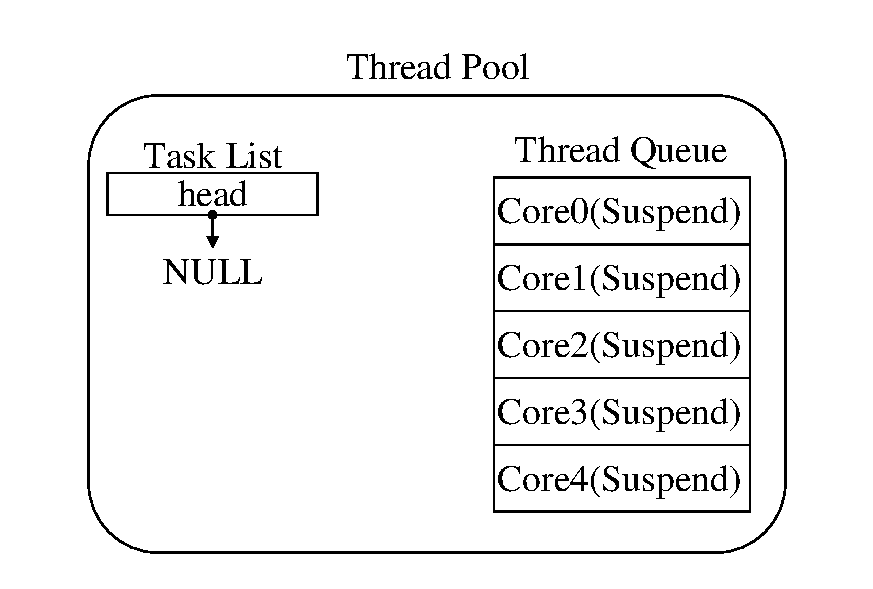
\includegraphics[width = .6\textwidth]{init.pdf}
	\caption{初始化线程池}
\end{figure}
\begin{figure}[H]
	\centering
	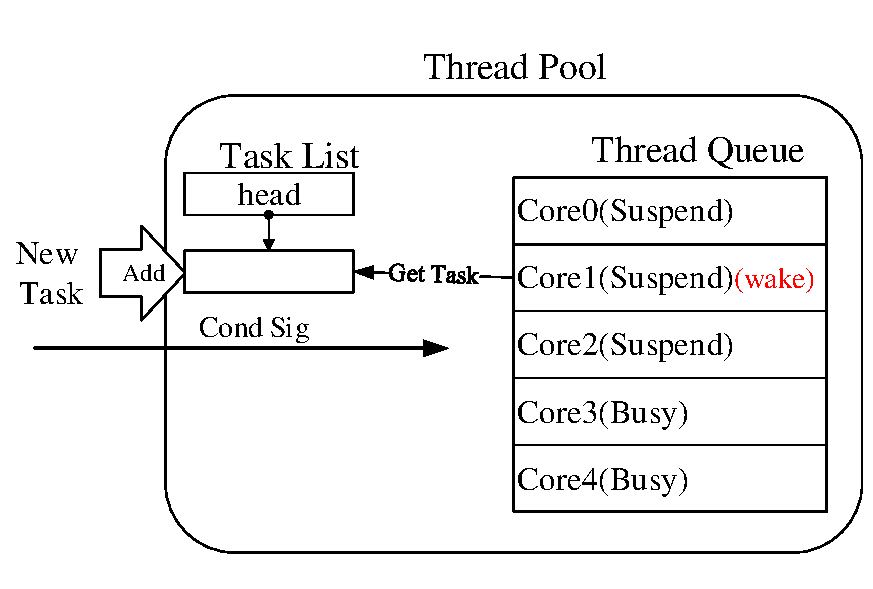
\includegraphics[width = .6\textwidth]{suspend.pdf}
	\caption{有线程挂起时}
\end{figure}
\begin{figure}[H]
	\centering
	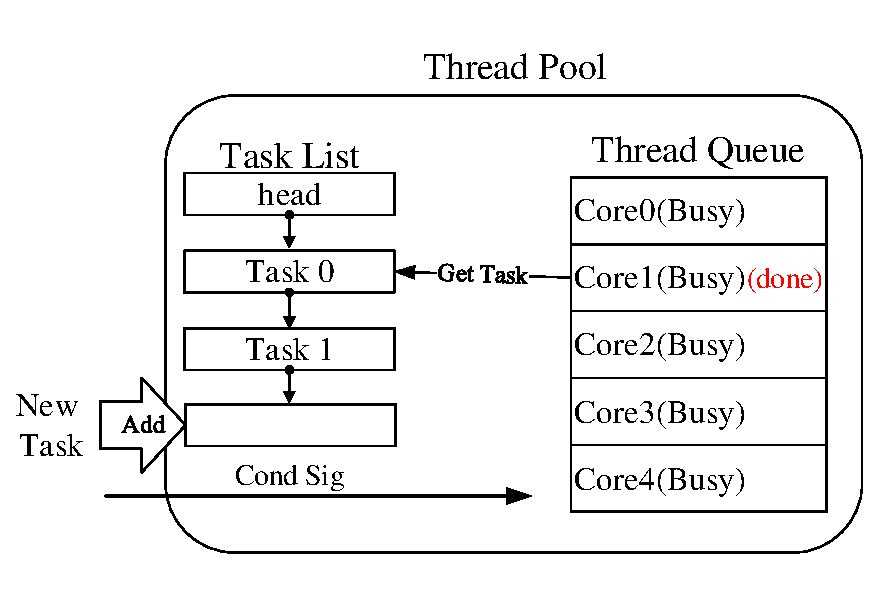
\includegraphics[width = .6\textwidth]{busy.pdf}
	\caption{线程全忙时}
\end{figure}
\subsection{线程池的优势}
1. 动态分配CPU核心;\\
2. 限制线程运行核心位置;\\
3. 避免重复创建和销毁线程。

%===========第三节=================
\section{两种新的调度方案}
\subsection{轮询方案(不使用信号量)}
\begin{figure}[H]
	\centering
	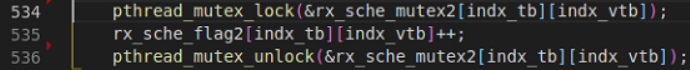
\includegraphics[width = \textwidth]{poll0.png}
	\caption{关键步骤}
\end{figure}
\begin{figure}[H]
	\centering
	\begin{minipage}[t]{0.48\textwidth}
		\centering
		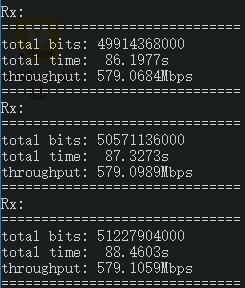
\includegraphics[width = \textwidth]{pollsta.png}
		\caption{轮询方案性能}
	\end{minipage}
	\begin{minipage}[t]{0.48\textwidth}
		\centering
		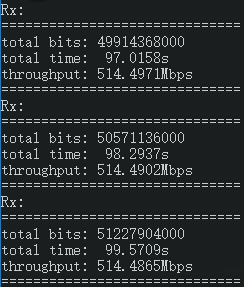
\includegraphics[width = \textwidth]{semsta.png}
		\caption{信号量方案性能}
	\end{minipage}
\end{figure}
\subsection{不使用线程池}
\begin{figure}[H]
	\centering
	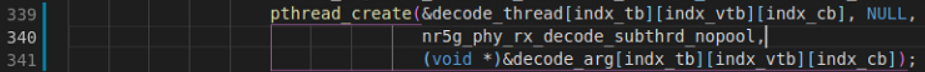
\includegraphics[width = \textwidth]{nopool0.png}
	\caption{关键步骤}
\end{figure}
\begin{figure}[H]
	\centering
	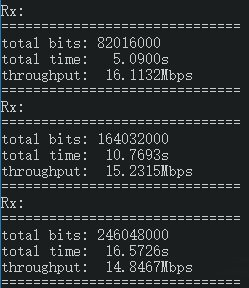
\includegraphics[width = .4\textwidth]{nopool.png}
	\caption{性能}
\end{figure}

%===========第四节=================
\section{尝试修改线程池}
\subsection{线程池过大造成性能下降的问题}
\begin{figure}[H]
	\centering
	\begin{minipage}[t]{0.48\textwidth}
		\centering
		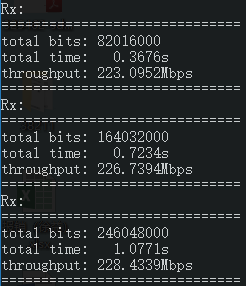
\includegraphics[width = \textwidth]{rxs42.png}
		\caption{单流4CPU2CORE}
	\end{minipage}
	\begin{minipage}[t]{0.48\textwidth}
		\centering
		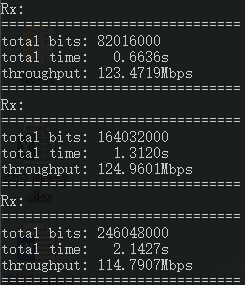
\includegraphics[width = \textwidth]{rxs414.png}
		\caption{单流4CPU14CORE}
	\end{minipage}
\end{figure}
\begin{figure}[H]
	\centering
	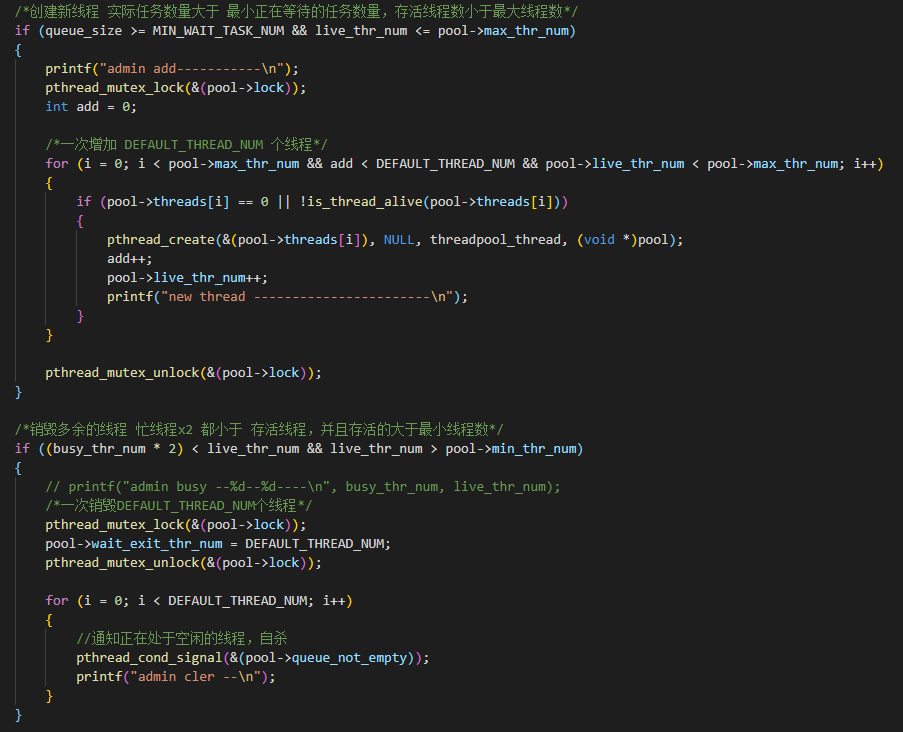
\includegraphics[width = \textwidth]{adm.png}
	\caption{动态调整线程池大小}
\end{figure}
\subsection{问题}
1. 每个线程池需要额外的管理线程;\\
2. 线程池大小调整过于频繁。

%===========第五节=================
% \section{修改开题报告}


%===========下周计划=================
\section{下阶段计划}
1. 尝试从文献中寻找新的线程池方案;

2. 完善PHY-MAC接口(包括链路自适应和分块重传部分)。

\end{document}
%%%%%%%%%%%%%%%%%%%%%%%这是正文部分的结束%%%%%%%%%%%%